\section{Global force approximation error}
The situation portrayed in \autoref{fig:reference-force-approx-different-schemes} gives insight into a field due to a single particle.
In a typical situation, we are interested in simulating many thousands of particles, and thus, the averaged approximation error becomes of interest.
Just as in the case of the PM method, the global error was measured in terms of mean relative error given by \autoref{eq:force-avg-relative-err}.
This time, the error was plotted as a function of the particle diameter for both TSC and NGP schemes in two variants, using second-order and fourth-order Laplacian approximations.
The result of this test is shown in \autoref{fig:reference-force-error-different-schemes-sub}.
The figure illustrates that the error decays rapidly with increasing particle diameter when the TSC scheme is used.
It is worth noting that the fourth-order accurate finite difference yields significant improvement in accuracy for the TSC scheme-based P3M method, allowing the error to drop below $1\%$ mark for $a \approx 4H$.

The ``local picture'' of the errors of force approximation in the \PThreeM{} method has already been outlined in \autoref{fig:reference-force-combined}.
Now we turn to investigate how the choice of the particle shape ($S_1$ or $S_2$) and the size of the particle diameter influence the global force approximation error.
The error is defined the same as in the case of the PM method, i.e., we use \autoref{eq:force-avg-relative-err}.

In our test, the grid covering the computational region had dimensions of $64\times 64\times 32$, and $N=10{,}000$ particles were used.
The result of the test is shown in \autoref{fig:p3m-global-err-combined}.
\begin{figure}[htp]
    \centering
    \begin{subfigure}[b]{0.48\textwidth}
        \centering
        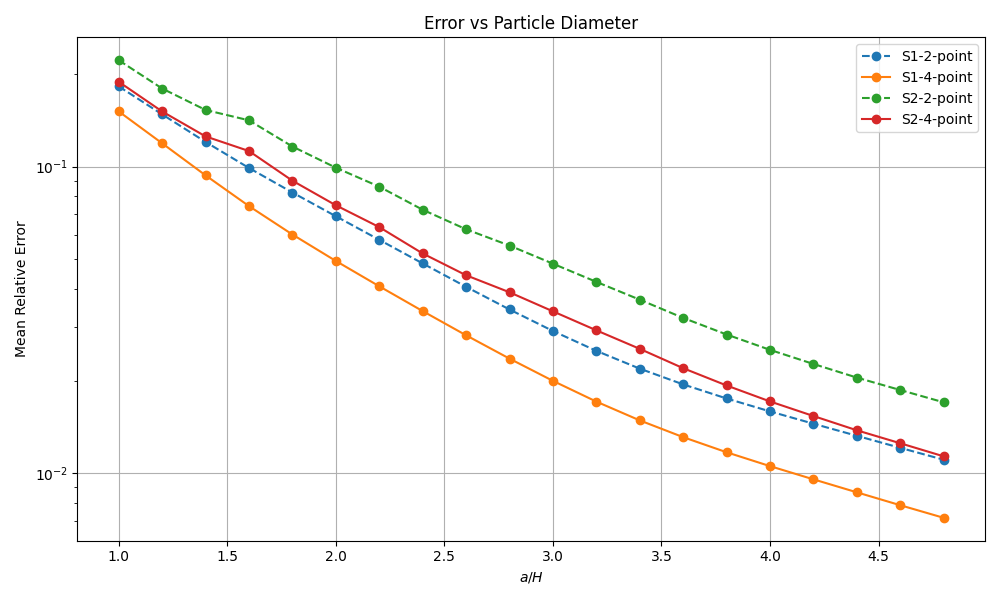
\includegraphics[width=\textwidth]{chapters/p3m-method/img/err_vs_part_diam_p3m.png}
        \caption{Mean error for different particle shapes.}
        \label{fig:reference-force-approx-different-shapes-sub}
    \end{subfigure}
    \hfill
    \begin{subfigure}[b]{0.48\textwidth}
        \centering
        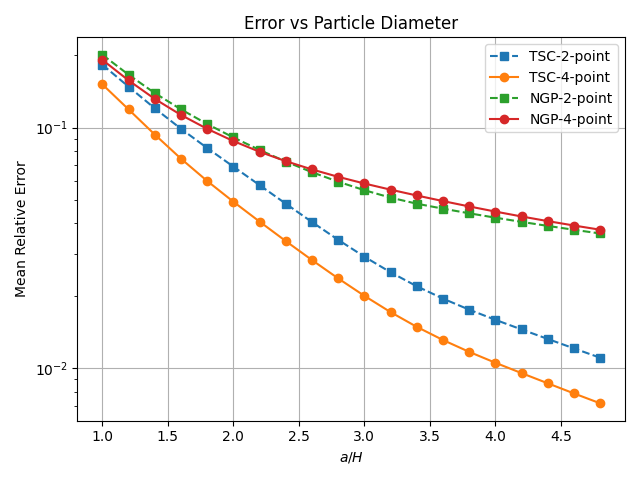
\includegraphics[width=\textwidth]{chapters/p3m-method/img/no-cic.png}
        \caption{Mean error for different assignment schemes.}
        \label{fig:reference-force-error-different-schemes-sub}
    \end{subfigure}
    \caption{Comparison of PM approximation using different assignment and interpolation functions.
    In the test we set $N=10{,}000$ and used $64\times 64\times 32$ grid.
    }
    \label{fig:p3m-global-err-combined}
\end{figure}
The figure clearly illustrates that the error drops with increasing the size of the particle diameter $a$, which is an expected result, as the P3M method calculates more interparticle forces with increasing $ a$ through exact direct summation.
Moreover, as we could see in \autoref{fig:reference-force-error-sub}, the PM approximation to the reference force gets better with increasing particle diameter.
These two effects combined are responsible for the reduction of global error.

For both the $S_1$ and $S_2$ shapes, the error was minimized when the fourth-order finite difference was used for gradient calculation, as one could expect.
The test indicated the superiority of the $S_1$ shape, with the difference between the two becoming more significant for bigger relative values of $a$.